\documentclass{scrreprt}
\usepackage{listings}
\usepackage{underscore}
\usepackage{graphicx}
\usepackage[bookmarks=true]{hyperref}
\usepackage[utf8]{inputenc}
\usepackage[T1]{fontenc}
\usepackage[english,russian]{babel}
\hypersetup{
    unicode=true,
    bookmarks=false,    % show bookmarks bar?
    pdftitle={Software Requirement Specification},    % title
    pdfauthor={Jean-Philippe Eisenbarth},                     % author
    pdfsubject={TeX and LaTeX},                        % subject of the document
    pdfkeywords={TeX, LaTeX, graphics, images}, % list of keywords
    colorlinks=true,       % false: boxed links; true: colored links
    linkcolor=blue,       % color of internal links
    citecolor=black,       % color of links to bibliography
    filecolor=black,        % color of file links
    urlcolor=purple,        % color of external links
    linktoc=page            % only page is linked
}
\usepackage{hyperref}
\def\vCurrentVersion{v0.1.0 }
\def\vProjectName{simple-routine}


\begin{document}

\begin{flushright}
    \rule{16cm}{5pt}\vskip1cm
    \begin{bfseries}
        \Huge{СПЕЦИФИКАЦИЯ ТРЕБОВАНИЙ\\ К ПРОЕКТУ}\\
        \vspace{3.0cm}
        \huge{<<\vProjectName>>}\\
        \vspace*{\fill}
        \LARGE{\vCurrentVersion}\\
        \today\\
    \end{bfseries}
\end{flushright}

\tableofcontents

\chapter*{История изменений}

\begin{center}
    \begin{tabular}{|c|c|c|}
        \hline
	    Дата & Описание изменений & Версия\\
        \hline
        02.03.2021 & Описание основных разделов спецификации & 0.1.0 \\
        \hline
    \end{tabular}
\end{center}
\chapter{Введение}
\section{Цели}
Данный документ описывает приложение <<\vProjectName>> --- инструмент для ежедневнего планирования. Основные цели приложения --- помочь пользователю отслеживать выполнение рутинных задач, а также способствовать достижению долгосрочных целей.

\section{Соглашения о терминах}
\begin{itemize}
    \item \textbf{Цель} --- масштабная задача, имеющая срок выполнения и план действий к ее достижению.
    \item \textbf{Список задач} --- план необходимых действий для достижения \textbf{цели}.
    \item \textbf{Задача} --- атомарное действие, составляющее \textbf{список задач}.
    \item \textbf{Календарь} --- инструмент для составления персонального расписания выполнения \textbf{задач} внутри приложения.
    \item \textbf{Помодорро} --- таймер длительностью на усмотрение пользователя (по умолчанию --- 25 минут) для сконцентрированной работы над \textbf{задачей}.
    \item \textbf{Шаблон} --- автоматическое создание в \textbf{календаре} заданного пользователем количества копий \textbf{задач} для удобного соблюдения их регулярного выполнения.
\end{itemize}


\section{Предполагаемая аудитория}
Данный документ предназначен для команды разработки проекта <<\vProjectName>>, а именно для разработчиков, менеджеров проекта, тестировщиков, а также для будущих пользователей приложения. Общее видение продукта и основные характеристики представлены в разделе \ref{ch:description} и будут интересны потенциальным пользователям. В разделах \ref{ch:functionality} и \ref{ch:nonfunctional} представлены функциональные и нефункциональные требования, интересные разработчикам и тестировщикам продукта, а также прочие требования, которые могут заинтересовать менеджеров проекта. 

\section{Масштаб проекта}
Изначальная минимальная версия приложения предназначена для русскоязычных пользователей. В дальнейшем возможно расширение продукта и его вывод на международный рынок.

\section{Ссылки на источники}
https://github.com/egorklimov/simple-routine
\chapter{Общее описание}
\label{ch:description}
\section{Видение продукта}
<<\vProjectName>>  --- новый продукт, объединяющий в себе характеристики многих полезных инструментов повседневного использования. Существуют удобные инструменты для отдельных компонентов этого приложения: календарь (Google календарь), заметки (Evernote), трекер привычек (Productive), отслеживане достижения целей (Trello), список задач (Todoist). Однако на данный момент нет приложения, удобным образом объединяющего в себе все необходимые инструменты. simple-routine задуман именно таким.


\section{Функциональность продукта}
\begin{itemize}
    \item ежедневный трекер привычек
    \item календарь с напоминаниями о созданных событиях
    \item доска канбан для выполнения длительных и/или многоступенчатых задач
    \item таймер продуктивности <<помодорро>>
    \item анализ эффективности выполнения задач и следования планам
    \item возможность делиться результатами с другими пользователями
\end{itemize}


\section{Классы и характеристики пользователей}
Приложение подойдет для людей разных возрастных групп. Оно будет полезно для тех, кто хочет успевать больше, кто не хочет/не может держать все цели и задачи в голове, а хочет зафиксировать их в удобном месте и планомерно двигаться к их достижению. Шаблоны будут полезны для тех, кто хочет выработать определенные привычки, а таймер <<помодорро>> --- для тех, кому сложно сосредоточиться на рутинных или больших задачах. Проект планируется интернациональным, с первоначальным релизом на русскоязычную аудиторию.

\section{Среда функционирования продукта}
simple-routine --- облачный веб-сервис, разрабатываемый с использованием технологии Progressive Web App (PWA), для поддержания различных платформ (ПК/мобильное приложение/адаптивный веб-сайт). Приложение должно легко адаптироваться к росту нагрузки, а также не должно зависить от среды выполнения, поэтому выбран cloud native подход. Сервис должен корректно работать в условиях ухудшения и полной потери связи, для поддержания <<офлайн режима>> планируется использовать механизм service worker.

\section{Рамки, ограничения, правила и стандарты}
\begin{itemize}
    \item Приложение ориентировано на персональное и командное использование. Таким образом, приложение не предполагает доступ к информации неограниченного круга лиц, поэтому не является СМИ согласно Закону РФ от 27.12.1991 N 2124-1 (ред. от 30.12.2020) "О средствах массовой информации" (с изм. и доп., вступ. в силу с 01.01.2021. Перед интернационализацией сервиса необходимо оценить требования регуляторов других стран. Опицонально, можно поддержать внутреннюю социальную сеть, однако, эта возможность не входит в список минимальных требований для запуска продукта и требует дополнительного анализа ограничений, т.к. в таком случае сервис может быть приравнен к СМИ.
    \item К правилам относится неразглашение личной информации пользователя, его целей и событий календаря. 
    \item Сервис должен быть доступен людям с ограниченными возможностями (ГОСТ Р 52872-2019, Web Content Accessibility Guidelines)
\end{itemize}

\chapter{Функциональность системы}
\label{ch:functionality}

\begin{itemize}
\item ежедневный трекер привычек
\item календарь с напоминаниями о созданных событиях
\item доска канбан для выполнения длительных и/или многоступенчатых задач
\item таймер продуктивности “помодоро”
\item анализ эффективности выполнения задач и следования планам
\item возможность делиться результатами с другими пользователями
\end{itemize}


\section{Ежедневный трекер привычек}
Подойдет для выработки привычки. Приложение даст напоминание выполнить ежедневную запланированную деятельность в указанное время.

\subsection{Описание и приоритет}
Пользователь создает ежедневную задачу, которую хочет выполнять регулярно в течение заданного промежутка времени, чтобы выработать привычку. Приложение уведомляет пользователя и подбадривает на пути к достижению цели

\subsection{Функциональные требования}
Создание/удаление задачи, настройка уведомлений


\section{таймер продуктвиности <<помодоро>>}
Популярная методика для повышения продуктивности работы

\subsection{Описание и приоритет}
Установлено, что специальным образом установленные промежутки работы и отдыха, позволяют увеличить производительность работы. Таким образом таймер поможет пользователю соблюдать этот режим.

\subsection{Функциональные требования}
Настройка таймера, удобство его использования


\section{доска кабан}
Интерфейс, позволяющий визуализировать и структурировать работу в команде над крупными проектами.

\subsection{Описание и приоритет}
Представляет из себя доску, поделенную на этапы выполнения задач, помогает отслеживать ход их выполнения и контролировать процесс крупной задачи

\subsection{Функциональные требования}
Добавление задач, перемещение их по доске, подсчитанные статистики количества выполненной работы.


\section{календарь событий}

\subsection{Описание и приоритет}
Календарь, в который можно добавлять события и получать уведомления об их приближении

\subsection{Функциональные требования}
Добавление, удаление и редактирование событий, настройка уведомлений на них.
\chapter{Нефункциональные требования}
\label{ch:nonfunctional}

\section{Требования к окружению}
Среда функционирования ПО описана в разделе \ref{sec:environment}.\\ <<simple-routine>> - \href{https://github.com/cncf/toc/blob/main/DEFINITION.md#\%D1\%80\%D1\%83\%D1\%81\%D1\%81\%D0\%BA\%D0\%B8\%D0\%B9}{\color{blue}{cloud native}} приложение и должно соответствовать стандартам Cloud Native Computing Foundation. 

Оркестрация должна быть реализована с использованием Kubernetes. Для поддержания высокого уровня доступности сервиса планируется воспользоваться услугами внешних провайдеров, таких как Amazon Web Services и Google Cloud, которые гарантируют высокий уровень качества предоставления услуг в своих соглашениях об уровне услуг (Service Level Agreement, SLA). Гарантированная доступность сервиса <<simple-routine>> должна соответствовать - 95\% в месяц. Для повышения уровня доверия к сервису необходимо сформировать SLA и предоставить его пользователям на основной странице сервиса. 

Необходим режим с пониженным использованием интернет-трафика --- для экономии интернет-трафика пользователя, в таком режиме пользователь должен иметь возможность увидеть объем потребляемого трафика, а также изменить качество вспомогательных элементов (картинки, стили).

\section{Требования к производительности}
Приложение должно эффективно работать на смартфоне, а также на ПК. Страницы web-приложения должны загружаться не дольше 3х секунд. Отклик для мобильного приложения должен составлять не больше секунды. Среднее значение статистик при прохождении анализатора \href{https://developers.google.com/web/tools/lighthouse}{\color{blue}{Google Lighthouse}} должно быть не меньше 95.


\section{Требования к сохранности (данных)}
\begin{itemize}
    \item Процесс аутентификации должен соответствовать стандарту OAuth 2.0, с поддержкой формата токена JSON Web Token (JWT);
    \item Чувствительные пользовательские данные должны должны храниться в зашифрованном виде;
    \item Необходимо гарантировать восстановление пользовательских данных за последние 8 часов работы сервиса при условии падения сервиса;
    \item Способность к резервному копированию данных;
    \item Архивирование действий пользователей и системных событий;
    \item Данные внесенные в <<офлайн режиме>> должны быть синхронизированы с хранилищем при восстановлении связи.
\end{itemize}

\section{Критерии качества ПО}
\begin{itemize}
    \item Возможность установки через GooglePlay с устройства, а также через ПК;
    \item Отсутствие утечек памяти;
    \item Низкий уровень потребления энергии при работе в фоновом режиме;
    \item Выполнение описанных в документе функциональных и нефункциональных требований;
    \item Уровень тестового прокрытия - 85\%;
    \item Прохождение статических анализаторов кода;
    \item Высокий уровень мониторинга работы сервиса и поддержание трассировки пользовательских запросов в серсиве (с использованием стандарта OpenTelemetry).
\end{itemize}


\section{Требования к безопасности системы}
Приложение должно поддерживать шифрование персональных данных пользователей при записи в память во избежание утечки информации. Необходима строгая аутентификация и авторизация, а также привязка процессов внутри приложения к идентификатору пользователя. В случае нарушения безопасности системы необходимо иметь возможность точно оценить уровень утечки и оперативно уведомить пользователей. 


\section{Прочие требования}

Все основые требования описаны в разделах \ref{ch:functionality} и \ref{ch:nonfunctional}.
\chapter{Приложения}
\section{Приложение A: Диаграмма использования}
\begin{figure}[h]
    \centering
    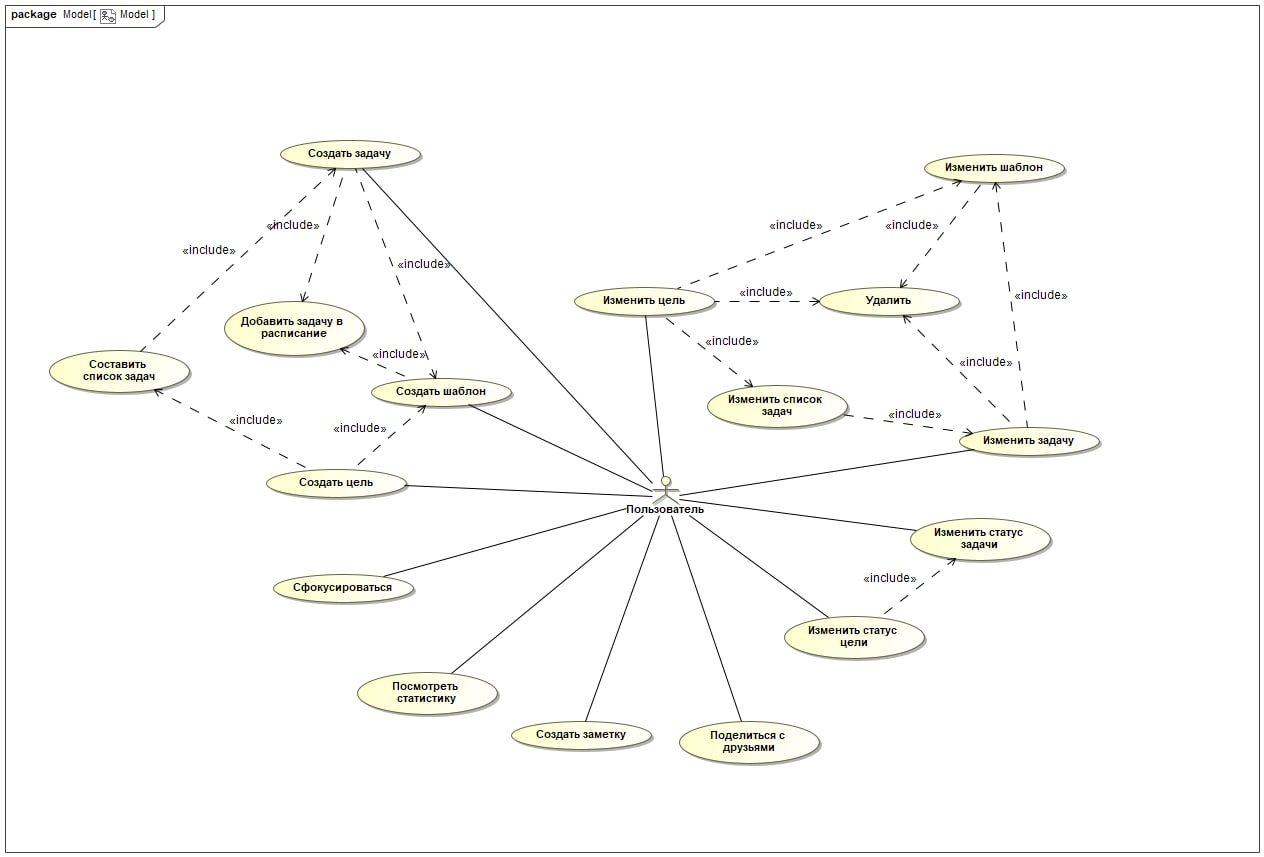
\includegraphics[angle=90,height=0.7\textheight]{img/use-case-diagram.jpg}
    \caption{Диаграмма использования} 
    \label{fig:use_case_diagram}
\end{figure}

\newpage
\section{Приложение B: Диаграмма требований}
\begin{figure}[h]
    \centering
    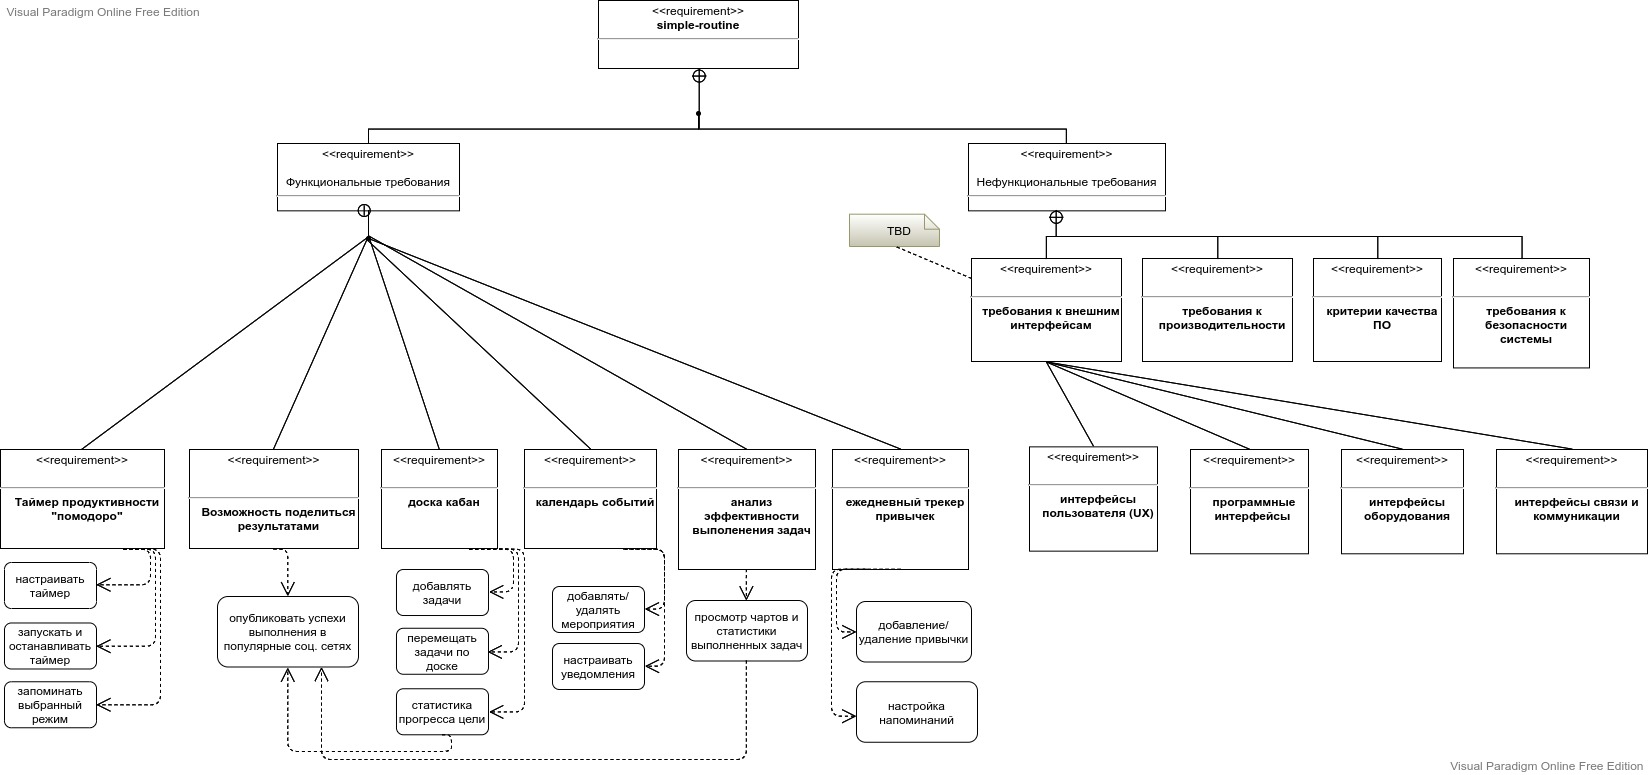
\includegraphics[angle=90,height=0.7\textheight,width=0.6\textwidth]{img/requirement-diagram.jpg}
    \caption{Диаграмма требований} 
    \label{fig:requirement_diagram}.
\end{figure}


\end{document}